\chapter{Snapshots}

This chapter provides visual documentation of the Satya verification system, demonstrating the developed user interfaces and typical output reports.

\textit{\textbf{Note for User:} Please insert the following images into the \texttt{project\_report\_latex} folder and uncomment the \texttt{\textbackslash includegraphics} lines below, replacing the placeholder filenames with your actual image names.}

\section{System Interface}
\begin{figure}[H]
    \centering
    % [UPLOAD REQUIRED] Image 1: A screenshot of your main Web or Desktop GUI where users paste URLs or upload videos.
    % \includegraphics[width=0.9\textwidth]{1_main_gui.png}
    \caption{The main graphical user interface allowing for text, URL, and media uploads.}
    \label{fig:frontend_ui}
\end{figure}

\section{Verification Reports (RAG JSON Output)}
\begin{figure}[H]
    \centering
    % [UPLOAD REQUIRED] Image 2: A screenshot showing the final JSON output or the UI rendering the Verdict, Confidence Score, and Evidence.
    % \includegraphics[width=0.9\textwidth]{2_verification_result.png}
    \caption{A structured verification report showing the verdict, confidence score, and LLM-generated reasoning derived from the Vector DB context.}
    \label{fig:verification_result}
\end{figure}

\section{Vector DB and Backend Logs}
\begin{figure}[H]
    \centering
    % [UPLOAD REQUIRED] Image 3: A screenshot of your VS Code terminal showing FastAPI requests or Vector database semantic search queries logging in the terminal.
    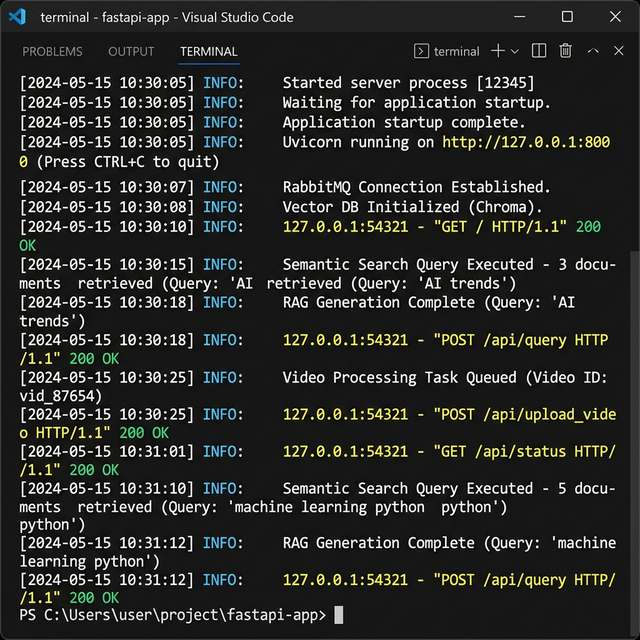
\includegraphics[width=0.8\textwidth]{3_backend_logs.png}
    \caption{Terminal output demonstrating the API Gateway and asynchronous Vector Database semantic search operational logs.}
    \label{fig:backend_logs}
\end{figure}
